\section{Function\-Bar Class Reference}
\label{classFunctionBar}\index{FunctionBar@{FunctionBar}}
{\tt \#include $<$functionbar.h$>$}

Inheritance diagram for Function\-Bar:\begin{figure}[H]
\begin{center}
\leavevmode
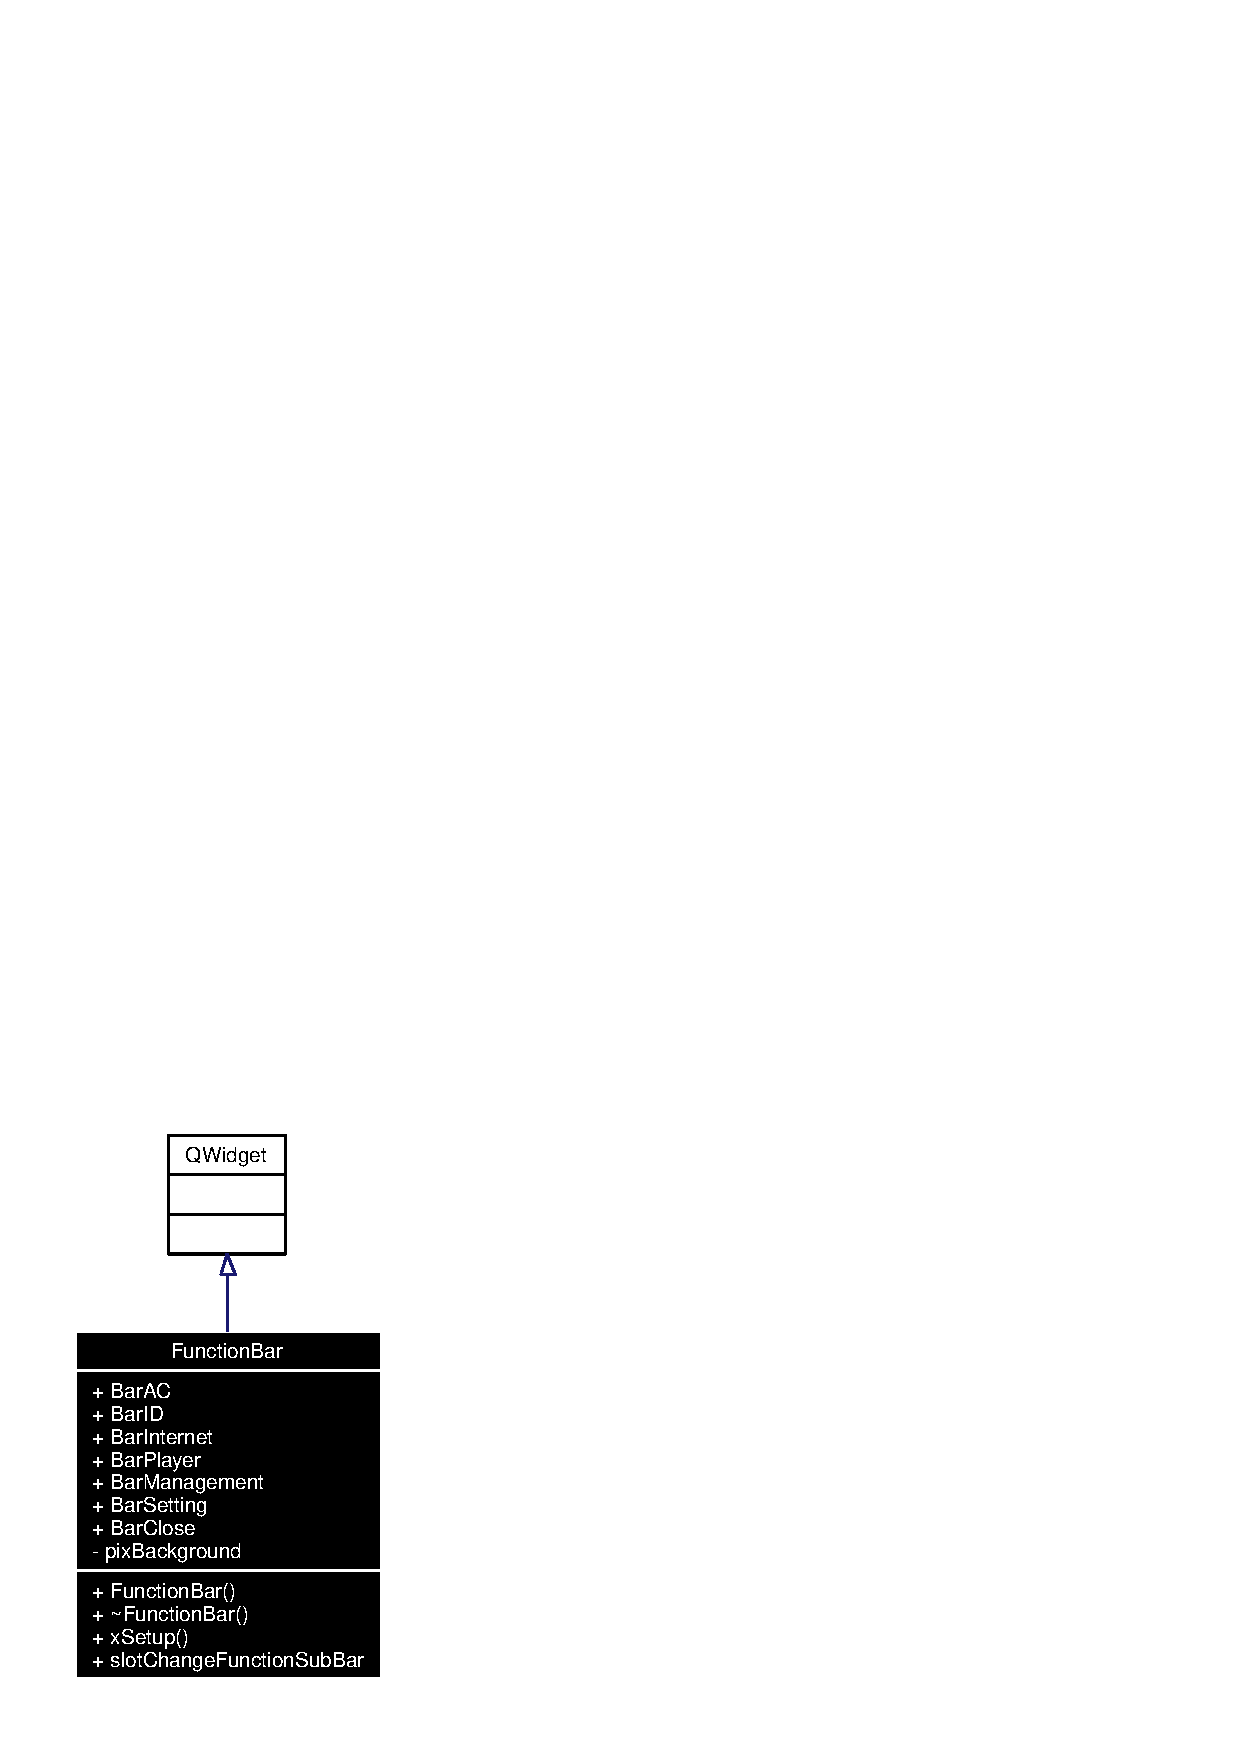
\includegraphics[width=91pt]{classFunctionBar__inherit__graph}
\end{center}
\end{figure}
Collaboration diagram for Function\-Bar:\begin{figure}[H]
\begin{center}
\leavevmode
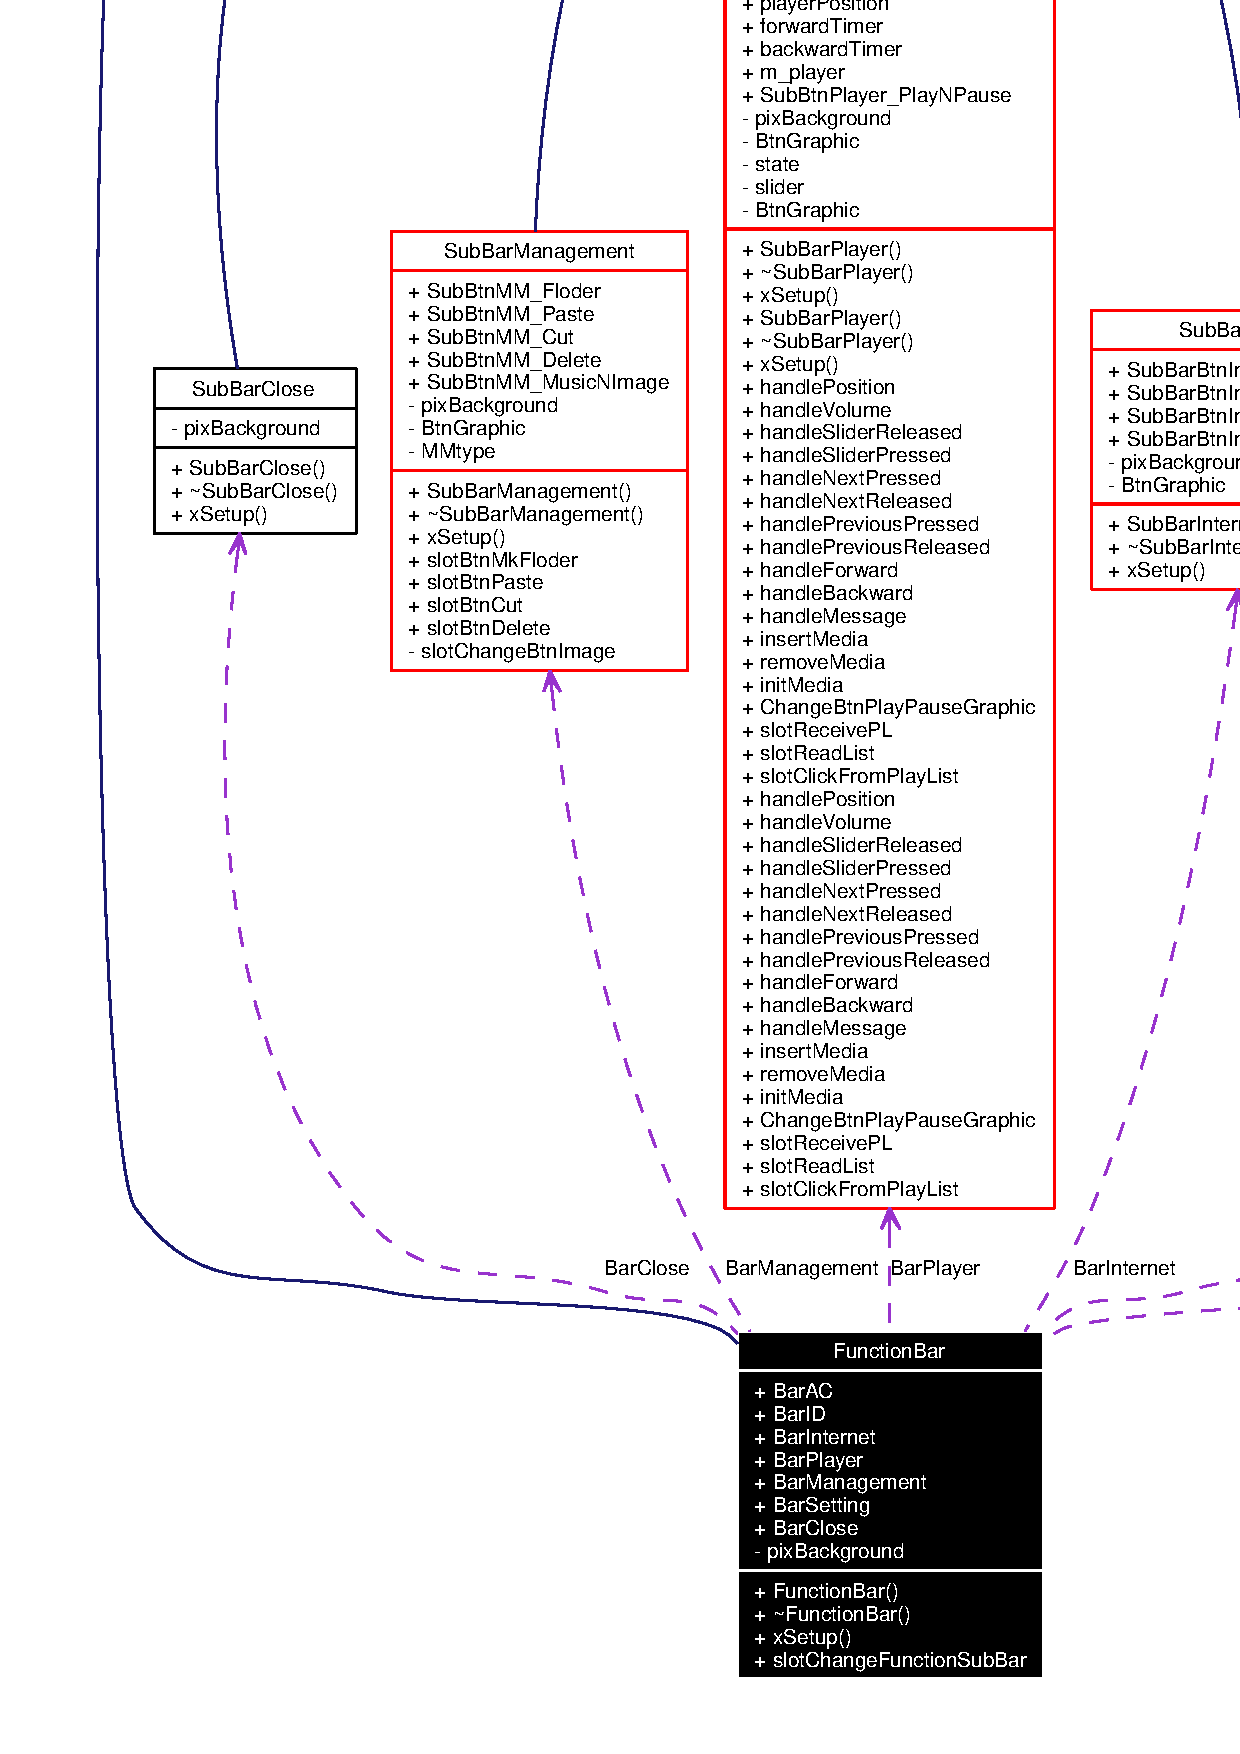
\includegraphics[width=420pt]{classFunctionBar__coll__graph}
\end{center}
\end{figure}


\subsection{Detailed Description}
\begin{Desc}
\item[Author:]sonicat \end{Desc}




Definition at line 37 of file functionbar.h.\subsection*{Public Slots}
\begin{CompactItemize}
\item 
void {\bf slot\-Change\-Function\-Sub\-Bar} (int)
\end{CompactItemize}
\subsection*{Signals}
\begin{CompactItemize}
\item 
void {\bf siganl\-Change\-Display\-Area\-Mode} (int)
\end{CompactItemize}
\subsection*{Public Member Functions}
\begin{CompactItemize}
\item 
{\bf Function\-Bar} ({\bf QWidget} $\ast$parent=0, const char $\ast$name=0)
\item 
{\bf $\sim$Function\-Bar} ()
\item 
void {\bf x\-Setup} ()
\end{CompactItemize}
\subsection*{Public Attributes}
\begin{CompactItemize}
\item 
{\bf Sub\-Bar\-Album\-Clock} $\ast$ {\bf Bar\-AC}
\item 
{\bf Sub\-Bar\-Album\-Clock} $\ast$ {\bf Bar\-ID}
\item 
{\bf Sub\-Bar\-Internet} $\ast$ {\bf Bar\-Internet}
\item 
{\bf Sub\-Bar\-Player} $\ast$ {\bf Bar\-Player}
\item 
{\bf Sub\-Bar\-Management} $\ast$ {\bf Bar\-Management}
\item 
{\bf Sub\-Bar\-Setting} $\ast$ {\bf Bar\-Setting}
\item 
{\bf Sub\-Bar\-Close} $\ast$ {\bf Bar\-Close}
\end{CompactItemize}
\subsection*{Private Attributes}
\begin{CompactItemize}
\item 
QPixmap {\bf pix\-Background}
\end{CompactItemize}


\subsection{Constructor \& Destructor Documentation}
\index{FunctionBar@{Function\-Bar}!FunctionBar@{FunctionBar}}
\index{FunctionBar@{FunctionBar}!FunctionBar@{Function\-Bar}}
\subsubsection{\setlength{\rightskip}{0pt plus 5cm}Function\-Bar::Function\-Bar ({\bf QWidget} $\ast$ {\em parent} = 0, const char $\ast$ {\em name} = 0)}\label{classFunctionBar_FunctionBara0}




Definition at line 22 of file functionbar.cpp.

References x\-Setup().



\footnotesize\begin{verbatim}23  : QWidget(parent, name)
24 {
25    xSetup();
26 }
\end{verbatim}\normalsize 


Here is the call graph for this function:\begin{figure}[H]
\begin{center}
\leavevmode
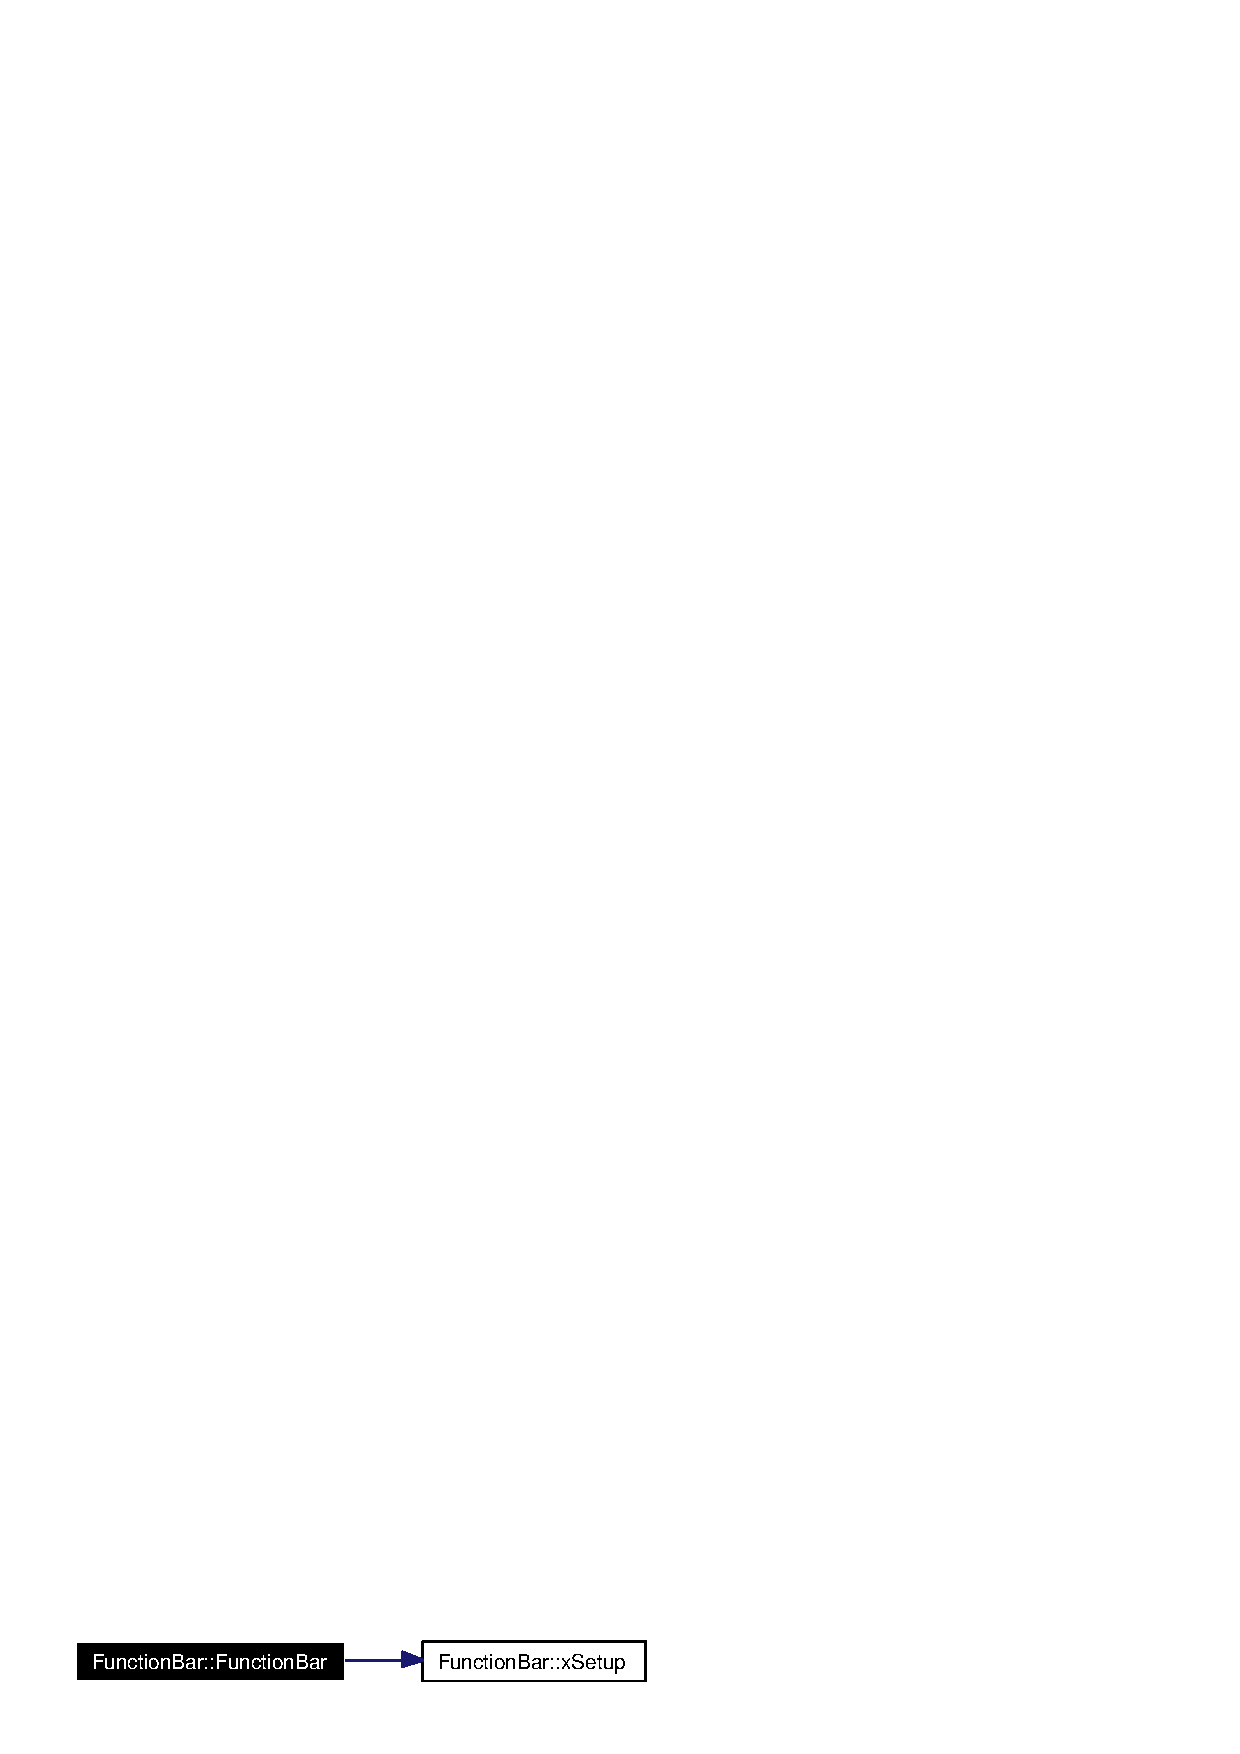
\includegraphics[width=155pt]{classFunctionBar_FunctionBara0_cgraph}
\end{center}
\end{figure}
\index{FunctionBar@{Function\-Bar}!~FunctionBar@{$\sim$FunctionBar}}
\index{~FunctionBar@{$\sim$FunctionBar}!FunctionBar@{Function\-Bar}}
\subsubsection{\setlength{\rightskip}{0pt plus 5cm}Function\-Bar::$\sim${\bf Function\-Bar} ()}\label{classFunctionBar_FunctionBara1}




Definition at line 29 of file functionbar.cpp.



\footnotesize\begin{verbatim}30 {
31 }
\end{verbatim}\normalsize 


\subsection{Member Function Documentation}
\index{FunctionBar@{Function\-Bar}!siganlChangeDisplayAreaMode@{siganlChangeDisplayAreaMode}}
\index{siganlChangeDisplayAreaMode@{siganlChangeDisplayAreaMode}!FunctionBar@{Function\-Bar}}
\subsubsection{\setlength{\rightskip}{0pt plus 5cm}void Function\-Bar::siganl\-Change\-Display\-Area\-Mode (int)\hspace{0.3cm}{\tt  [signal]}}\label{classFunctionBar_FunctionBarl0}




Definition at line 90 of file functionbar.moc.

Referenced by slot\-Change\-Function\-Sub\-Bar().



\footnotesize\begin{verbatim}91 {
92     activate_signal( staticMetaObject()->signalOffset() + 0, t0 );
93 }
\end{verbatim}\normalsize 
\index{FunctionBar@{Function\-Bar}!slotChangeFunctionSubBar@{slotChangeFunctionSubBar}}
\index{slotChangeFunctionSubBar@{slotChangeFunctionSubBar}!FunctionBar@{Function\-Bar}}
\subsubsection{\setlength{\rightskip}{0pt plus 5cm}void Function\-Bar::slot\-Change\-Function\-Sub\-Bar (int)\hspace{0.3cm}{\tt  [slot]}}\label{classFunctionBar_FunctionBari0}




Definition at line 79 of file functionbar.cpp.

References Bar\-AC, Bar\-Close, Bar\-ID, Bar\-Internet, Bar\-Management, Bar\-Player, Bar\-Setting, em\_\-albumclock, em\_\-close, em\_\-display\_\-close, em\_\-display\_\-internet, em\_\-display\_\-management, em\_\-display\_\-player, em\_\-display\_\-setting, em\_\-imagedetial, em\_\-internet, em\_\-management, em\_\-player, em\_\-setting, Global\-Setting, HDASSGlobal\-Setting::int\-HDASS\_\-ALBUMCLOCK\_\-STATE, HDASSGlobal\-Setting::int\-HDSS\_\-DISPLAY\_\-STATE, and siganl\-Change\-Display\-Area\-Mode().

Referenced by x\-Setup().



\footnotesize\begin{verbatim}80 {
81   #if TRACE
82   qWarning("slotChangeFunctionSubBar::%d",FuncMode);
83   #endif
84   if(FuncMode==em_internet)
85   {
86     BarInternet->show();
87     BarPlayer->hide();
88     BarManagement->hide();
89     BarAC->hide();
90     BarSetting->hide();
91     BarClose->hide();
92     BarID->hide();
93     //DAVID Change  DisplayArea Mode
94     GlobalSetting.intHDSS_DISPLAY_STATE=em_display_internet;
95     emit siganlChangeDisplayAreaMode(GlobalSetting.intHDSS_DISPLAY_STATE);    
96   }
97   else if(FuncMode==em_player)
98   {
99     BarInternet->hide();
100     BarPlayer->show();
101     BarManagement->hide();
102     BarAC->hide();
103     BarSetting->hide();
104     BarClose->hide();
105     BarID->hide();
106     //DAVID Change  DisplayArea Mode
107     GlobalSetting.intHDSS_DISPLAY_STATE=em_display_player;
108     emit siganlChangeDisplayAreaMode(GlobalSetting.intHDSS_DISPLAY_STATE);    
109   }
110   else if(FuncMode==em_management)
111   {
112     BarInternet->hide();
113     BarPlayer->hide();
114     BarManagement->show();
115     BarAC->hide();
116     BarSetting->hide();
117     BarClose->hide();
118     BarID->hide();
119     //DAVID Change  DisplayArea Mode
120     GlobalSetting.intHDSS_DISPLAY_STATE=em_display_management;
121     emit siganlChangeDisplayAreaMode(GlobalSetting.intHDSS_DISPLAY_STATE);    
122   
123   }
124   else if(FuncMode==em_albumclock)
125   {
126     BarInternet->hide();
127     BarPlayer->hide();
128     BarManagement->hide();
129     BarAC->show();
130     BarSetting->hide();
131     BarClose->hide();
132     BarID->hide();
133     //DAVID Change  DisplayArea Mode
134     emit siganlChangeDisplayAreaMode(GlobalSetting.intHDASS_ALBUMCLOCK_STATE+3);    
135   }
136   else if(FuncMode==em_setting)
137   {
138     BarInternet->hide();
139     BarPlayer->hide();
140     BarManagement->hide();
141     BarAC->hide();
142     BarSetting->show();
143     BarClose->hide();
144     BarID->hide();
145     //DAVID Change  DisplayArea Mode
146     GlobalSetting.intHDSS_DISPLAY_STATE=em_display_setting;
147     emit siganlChangeDisplayAreaMode(GlobalSetting.intHDSS_DISPLAY_STATE);    
148   }
149   else if(FuncMode==em_close)
150   {
151     BarInternet->hide();
152     BarPlayer->hide();
153     BarManagement->hide();
154     BarAC->hide();
155     BarSetting->hide();
156     BarClose->show();
157     BarID->hide();
158     //DAVID Change  DisplayArea Mode
159     GlobalSetting.intHDSS_DISPLAY_STATE=em_display_close;
160     emit siganlChangeDisplayAreaMode(GlobalSetting.intHDSS_DISPLAY_STATE);    
161   }
162    else if(FuncMode==em_imagedetial)
163   {
164     BarInternet->hide();
165     BarPlayer->hide();
166     BarManagement->hide();
167     BarAC->hide();
168     BarSetting->hide();
169     BarClose->hide();
170     BarID->show();
171   }
172 }
\end{verbatim}\normalsize 
\index{FunctionBar@{Function\-Bar}!xSetup@{xSetup}}
\index{xSetup@{xSetup}!FunctionBar@{Function\-Bar}}
\subsubsection{\setlength{\rightskip}{0pt plus 5cm}void Function\-Bar::x\-Setup ()}\label{classFunctionBar_FunctionBara2}




Definition at line 33 of file functionbar.cpp.

References Bar\-AC, Bar\-Close, Bar\-ID, Bar\-Internet, Bar\-Management, Bar\-Player, Bar\-Setting, Global\-Setting, HDASSGlobal\-Setting::int\-HDASS\_\-FUNCTION\_\-STATE, and slot\-Change\-Function\-Sub\-Bar().

Referenced by Function\-Bar().



\footnotesize\begin{verbatim}34 {
35    //DAVID Setup Background;
36    pixBackground.load("/root/kde_application/hdass08/skin/FunctionBarBackground.jpg");
37    setBackgroundPixmap(pixBackground);
38    
39    //DAVID Init BarInternet
40    BarInternet=new SubBarInternet(this);
41    BarInternet->setGeometry(115,0,550,80);
42    BarInternet->hide();
43    
44    //DAVID Init BarPlayer
45    BarPlayer=new SubBarPlayer(this);
46    BarPlayer->setGeometry(115,0,550,80);
47    BarPlayer->hide();
48    
49    //DAVID Init BarManagement
50    BarManagement=new SubBarManagement(this);
51    BarManagement->setGeometry(115,0,550,80);
52    BarManagement->hide();
53    
54    //DAVID Init BarAC
55    BarAC=new SubBarAlbumClock(this);
56    BarAC->setGeometry(115,0,550,80);
57    BarAC->hide();
58    
59    //DAVID Init SubBarSetting
60    BarSetting=new SubBarSetting(this);
61    BarSetting->setGeometry(115,0,550,80);
62    BarSetting->hide();
63    
64    //DAVID Init BarClose
65    BarClose=new SubBarClose(this);
66    BarClose->setGeometry(115,0,550,80);
67    BarClose->hide();
68    
69    //DAVID Init BarID ,ImageDetial
70    BarID=new SubBarAlbumClock(this);
71    BarID->setGeometry(115,0,550,80);
72    BarID->hide();
73    
74    //DAVID Set the Current Setting to the ba state
75    slotChangeFunctionSubBar(GlobalSetting.intHDASS_FUNCTION_STATE);
76    
77 }
\end{verbatim}\normalsize 


\subsection{Member Data Documentation}
\index{FunctionBar@{Function\-Bar}!BarAC@{BarAC}}
\index{BarAC@{BarAC}!FunctionBar@{Function\-Bar}}
\subsubsection{\setlength{\rightskip}{0pt plus 5cm}{\bf Sub\-Bar\-Album\-Clock}$\ast$ {\bf Function\-Bar::Bar\-AC}}\label{classFunctionBar_FunctionBaro0}




Definition at line 45 of file functionbar.h.

Referenced by slot\-Change\-Function\-Sub\-Bar(), HDASS08::x\-Setup(), and x\-Setup().\index{FunctionBar@{Function\-Bar}!BarClose@{BarClose}}
\index{BarClose@{BarClose}!FunctionBar@{Function\-Bar}}
\subsubsection{\setlength{\rightskip}{0pt plus 5cm}{\bf Sub\-Bar\-Close}$\ast$ {\bf Function\-Bar::Bar\-Close}}\label{classFunctionBar_FunctionBaro6}




Definition at line 50 of file functionbar.h.

Referenced by slot\-Change\-Function\-Sub\-Bar(), and x\-Setup().\index{FunctionBar@{Function\-Bar}!BarID@{BarID}}
\index{BarID@{BarID}!FunctionBar@{Function\-Bar}}
\subsubsection{\setlength{\rightskip}{0pt plus 5cm}{\bf Sub\-Bar\-Album\-Clock} $\ast$ {\bf Function\-Bar::Bar\-ID}}\label{classFunctionBar_FunctionBaro1}




Definition at line 45 of file functionbar.h.

Referenced by slot\-Change\-Function\-Sub\-Bar(), HDASS08::x\-Setup(), and x\-Setup().\index{FunctionBar@{Function\-Bar}!BarInternet@{BarInternet}}
\index{BarInternet@{BarInternet}!FunctionBar@{Function\-Bar}}
\subsubsection{\setlength{\rightskip}{0pt plus 5cm}{\bf Sub\-Bar\-Internet}$\ast$ {\bf Function\-Bar::Bar\-Internet}}\label{classFunctionBar_FunctionBaro2}




Definition at line 46 of file functionbar.h.

Referenced by slot\-Change\-Function\-Sub\-Bar(), HDASS08::x\-Setup(), and x\-Setup().\index{FunctionBar@{Function\-Bar}!BarManagement@{BarManagement}}
\index{BarManagement@{BarManagement}!FunctionBar@{Function\-Bar}}
\subsubsection{\setlength{\rightskip}{0pt plus 5cm}{\bf Sub\-Bar\-Management}$\ast$ {\bf Function\-Bar::Bar\-Management}}\label{classFunctionBar_FunctionBaro4}




Definition at line 48 of file functionbar.h.

Referenced by slot\-Change\-Function\-Sub\-Bar(), HDASS08::x\-Setup(), and x\-Setup().\index{FunctionBar@{Function\-Bar}!BarPlayer@{BarPlayer}}
\index{BarPlayer@{BarPlayer}!FunctionBar@{Function\-Bar}}
\subsubsection{\setlength{\rightskip}{0pt plus 5cm}{\bf Sub\-Bar\-Player}$\ast$ {\bf Function\-Bar::Bar\-Player}}\label{classFunctionBar_FunctionBaro3}




Definition at line 47 of file functionbar.h.

Referenced by slot\-Change\-Function\-Sub\-Bar(), HDASS08::x\-Setup(), and x\-Setup().\index{FunctionBar@{Function\-Bar}!BarSetting@{BarSetting}}
\index{BarSetting@{BarSetting}!FunctionBar@{Function\-Bar}}
\subsubsection{\setlength{\rightskip}{0pt plus 5cm}{\bf Sub\-Bar\-Setting}$\ast$ {\bf Function\-Bar::Bar\-Setting}}\label{classFunctionBar_FunctionBaro5}




Definition at line 49 of file functionbar.h.

Referenced by slot\-Change\-Function\-Sub\-Bar(), and x\-Setup().\index{FunctionBar@{Function\-Bar}!pixBackground@{pixBackground}}
\index{pixBackground@{pixBackground}!FunctionBar@{Function\-Bar}}
\subsubsection{\setlength{\rightskip}{0pt plus 5cm}QPixmap {\bf Function\-Bar::pix\-Background}\hspace{0.3cm}{\tt  [private]}}\label{classFunctionBar_FunctionBarr0}




Definition at line 56 of file functionbar.h.

The documentation for this class was generated from the following files:\begin{CompactItemize}
\item 
{\bf functionbar.h}\item 
{\bf functionbar.moc}\item 
{\bf functionbar.cpp}\end{CompactItemize}
